\subsection{Muons}
\label{subsec:obj_muon}


Muons are selected using the ``Tight'' and ``Loose'' offline cut-based definitions. Similar to electrons, ``Tight'' muons are used for semileptonic top-pair selection and ``Loose'' muons are used to veto events with extra muons. The variables and cuts defining the selections are listed in Table~\ref{tab:tightmuon}. PF-based isolation with $R=0.4$ and $\Delta\beta$ correction is used.

\begin{table}[!ht]
\centering
\begin{tabular}{|c|c|c|}
\hline
  Variable                                          & Loose WP & Tight WP \\
\hline
  PF-muon                                           & true     & true   \\
  global muon                                       & -        & true   \\
  global OR tracker muon                            & true     & -      \\
  $\chi^2/$ndof of global muon fit $<$              & -        & $10$   \\
  No. of muon chamber hit in global muon fit $\geq$ & -        & $1$    \\
  No. of muon stations with muon segments $\geq$    & -        & $2$    \\
  $|d_0|$ (cm) $<$                                  & -        & $0.2$  \\
  $|d_z|$ (cm) $<$                                  & -        & $0.5$  \\
  No. of pixel hits $>$                             & -        & $0$    \\
  No. of tracker layers with hits $>$               & -        & $5$    \\
  relative isolation $<$                            & $0.2$    & $0.12$ \\
\hline
\end{tabular}
\caption{Variables and thresholds that define ``Loose'' and ``Tight'' muons. ``-'' indicates the variable is not considered for that working point.}
\label{tab:tightmuon}
\end{table}

Muon selection efficiencies measured with the tag-and-probe method in data and in the Drell-Yan MC sample are shown in Fig.~\ref{fig:mulooseeff} and Fig.~\ref{fig:mutighteff}. The data-to-MC tight muon selection efficiency scale factors for muons with $\pt>30\:\GeV\:$ are computed in $\pt$-$|\eta|$ bins and are shown in Table~\ref{tab:mutight_sf} and Fig.~\ref{fig:mu_sf}. Scale factors for the loose muon selection are shown in Table~\ref{tab:muloose_sf} and Fig.~\ref{fig:mu_sf}, and computed down to the $10\:\GeV\: \pt$ range. The point with large uncertainty in the $100\:\GeV\: \pt$ bin is due to the small number of events contained in the MC failing ``probes" sample, with the negative weights causing an overall negative yield. We will proceed to handle this by specifying a minimum allowable yield of 0 events.


 \begin{table}[!ht]
 \centering
 \begin{tabular}{|c|c|c|c|}
 \hline
 &                          &                              &                           \\
 & $0.0 < |\eta| < 1.2$ & $1.2 < |\eta| < 2.1$ & $2.1 < |\eta| < 2.4$ \\
  &                          &                              &                           \\
 \hline
 $30 < \pt <  40$ &  $0.997 \pm  0.001$  &  $0.999 \pm  0.001$  &  $0.990 \pm  0.002$ \\
 \hline
 $40 < \pt <  50$ &  $0.994 \pm  0.001$  &  $0.995 \pm  0.001$  &  $0.991 \pm  0.002$ \\
 \hline
 $50 < \pt < 100$ &  $0.992 \pm  0.001$  &  $0.993 \pm  0.001$  &  $0.982 \pm  0.008$ \\
\hline
$100 < \pt < 150 $&  $0.985 \pm  0.005$  &  $0.986 \pm  0.006$  &  $1.001 \pm  0.017$ \\
 \hline
  $    \pt > 150$ &  $0.984 \pm  0.009$  &  $0.960 \pm  0.012$  &  $0.904 \pm  0.040$ \\
\hline
\end{tabular}
\caption{Tight muon selection efficiency scale factors for muons with $\pt>30\:\GeV\:$}
\label{tab:mutight_sf}
\end{table}

\begin{table}[!ht]
 \centering
 \begin{tabular}{|c|c|c|c|}
 \hline
 &                          &                              &                           \\
 & $0.0 < |\eta| < 1.2$ & $1.2 < |\eta| < 2.1$ & $2.1 < |\eta| < 2.4$ \\
  &                          &                              &                           \\
 \hline
 $10 < \pt <  15$ &  $1.012 \pm  0.012 $ &  $0.994 \pm  0.011$  &  $0.992 \pm  0.019$ \\
 \hline
 $15 < \pt<  20$ &  $0.982 \pm  0.007$  &  $0.981 \pm  0.007$  &  $0.993 \pm  0.013$ \\
 \hline
 $20 < \pt <  25$ &  $0.998 \pm  0.004$  &  $1.007 \pm  0.005$  &  $1.007 \pm  0.008$ \\
 \hline
 $25 <  \pt<  30$ &  $0.999 \pm  0.002$  &  $1.001 \pm  0.002$  &  $1.010 \pm  0.004$ \\
 \hline
 $30 < \pt<  40$ &  $1.002 \pm  0.001$  &  $1.002 \pm  0.001$  &  $1.001 \pm  0.001$ \\
 \hline
 $40 < \pt <  50$ &  $1.001 \pm  0.001$  &  $1.000 \pm  0.001$  &  $1.002 \pm  0.001 $\\
 \hline
 $50 <\pt < 100$ &  $1.000 \pm  0.001$  &  $0.999 \pm  0.001$  &  $1.001 \pm  0.001$ \\
 \hline
$100 < \pt< 150$ & $ 0.997 \pm  0.003$  &  $0.997 \pm  0.003$  &  $0.999 \pm  0.999$ \\
\hline
$\pt> 150$ &  $1.004 \pm  0.004$  &  $0.987 \pm  0.007 $ &  $1.000 \pm  0.008$ \\
\hline
\end{tabular}
\caption{Loose muon selection efficiency scale factors for muons with $\pt>10\:\GeV\:$}
\end{table}


\begin{figure}[htbp]
\begin{center}
  \subfigure[]{\label{sub fig:mutightsf}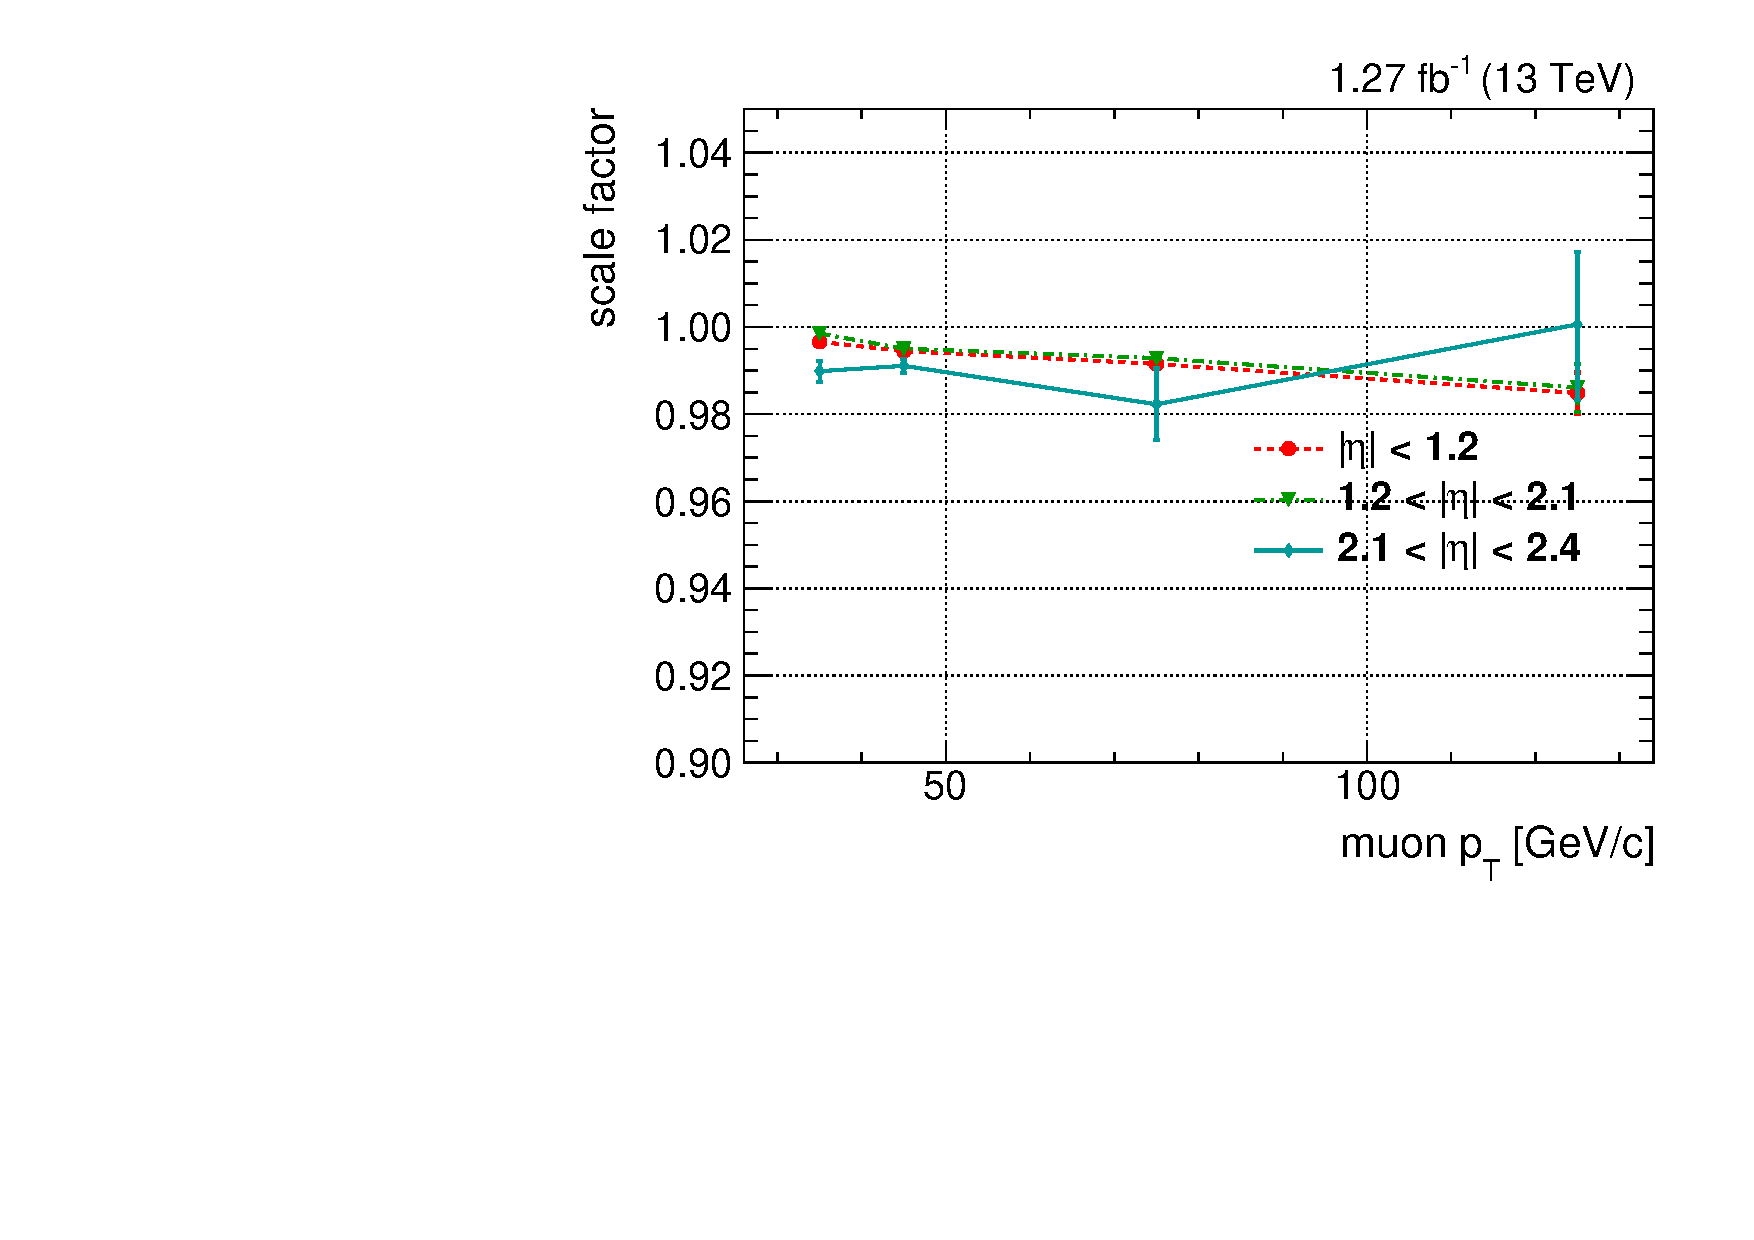
\includegraphics[width=0.48\textwidth]{figures/mutight_sfetapt.pdf}}	
  \subfigure[]{\label{sub fig:muloosesf}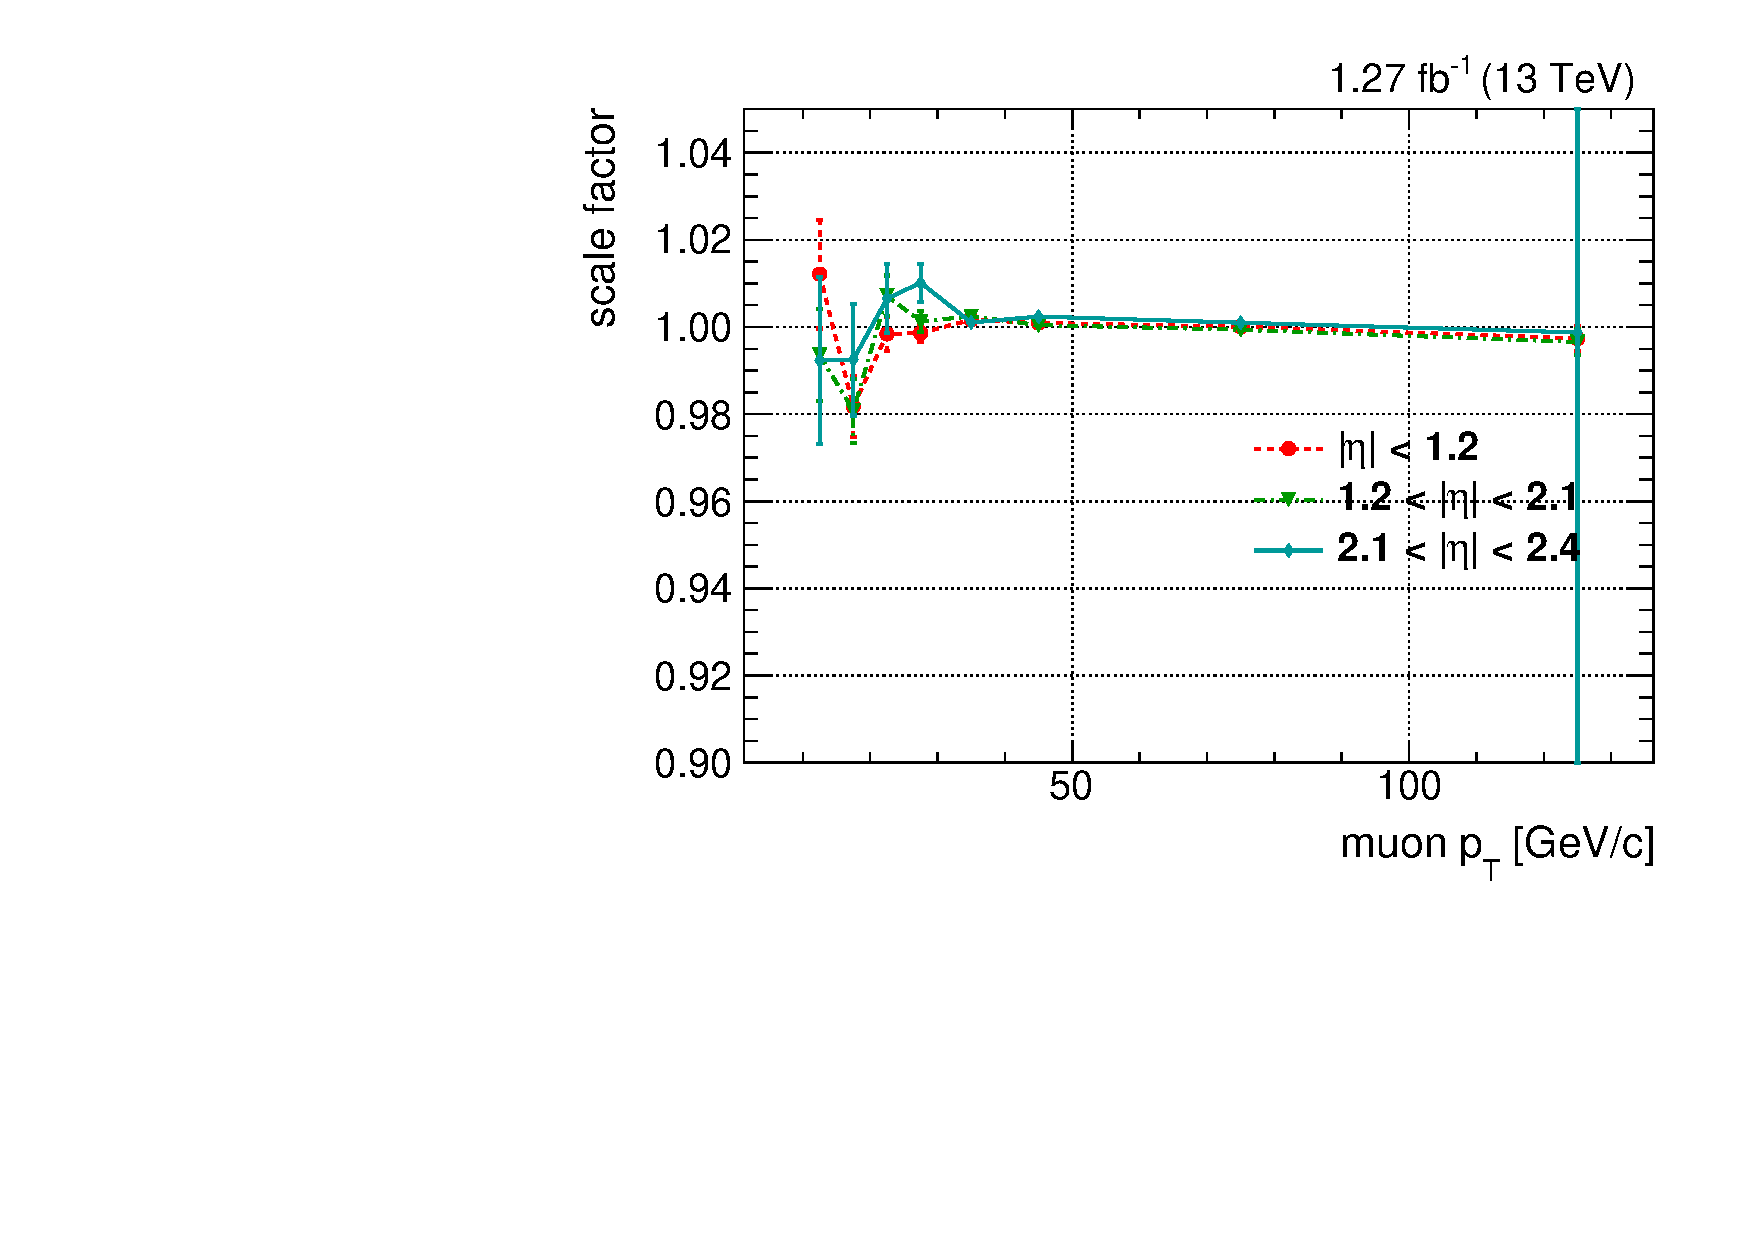
\includegraphics[width=0.48\textwidth]{figures/muloose_sfetapt.pdf}}
  \caption{Muon ``Tight" WP (left) and ``Loose" WP (right) data-to-MC efficiency scale factors as a function of muon $\pt$ for various $|\eta|$ bins.}
  \label{fig:mu_sf}
\end{center}
\end{figure}


\begin{figure}[htbp]
\begin{center}
  \subfigure[]{\label{subfig:mulooseeffeta}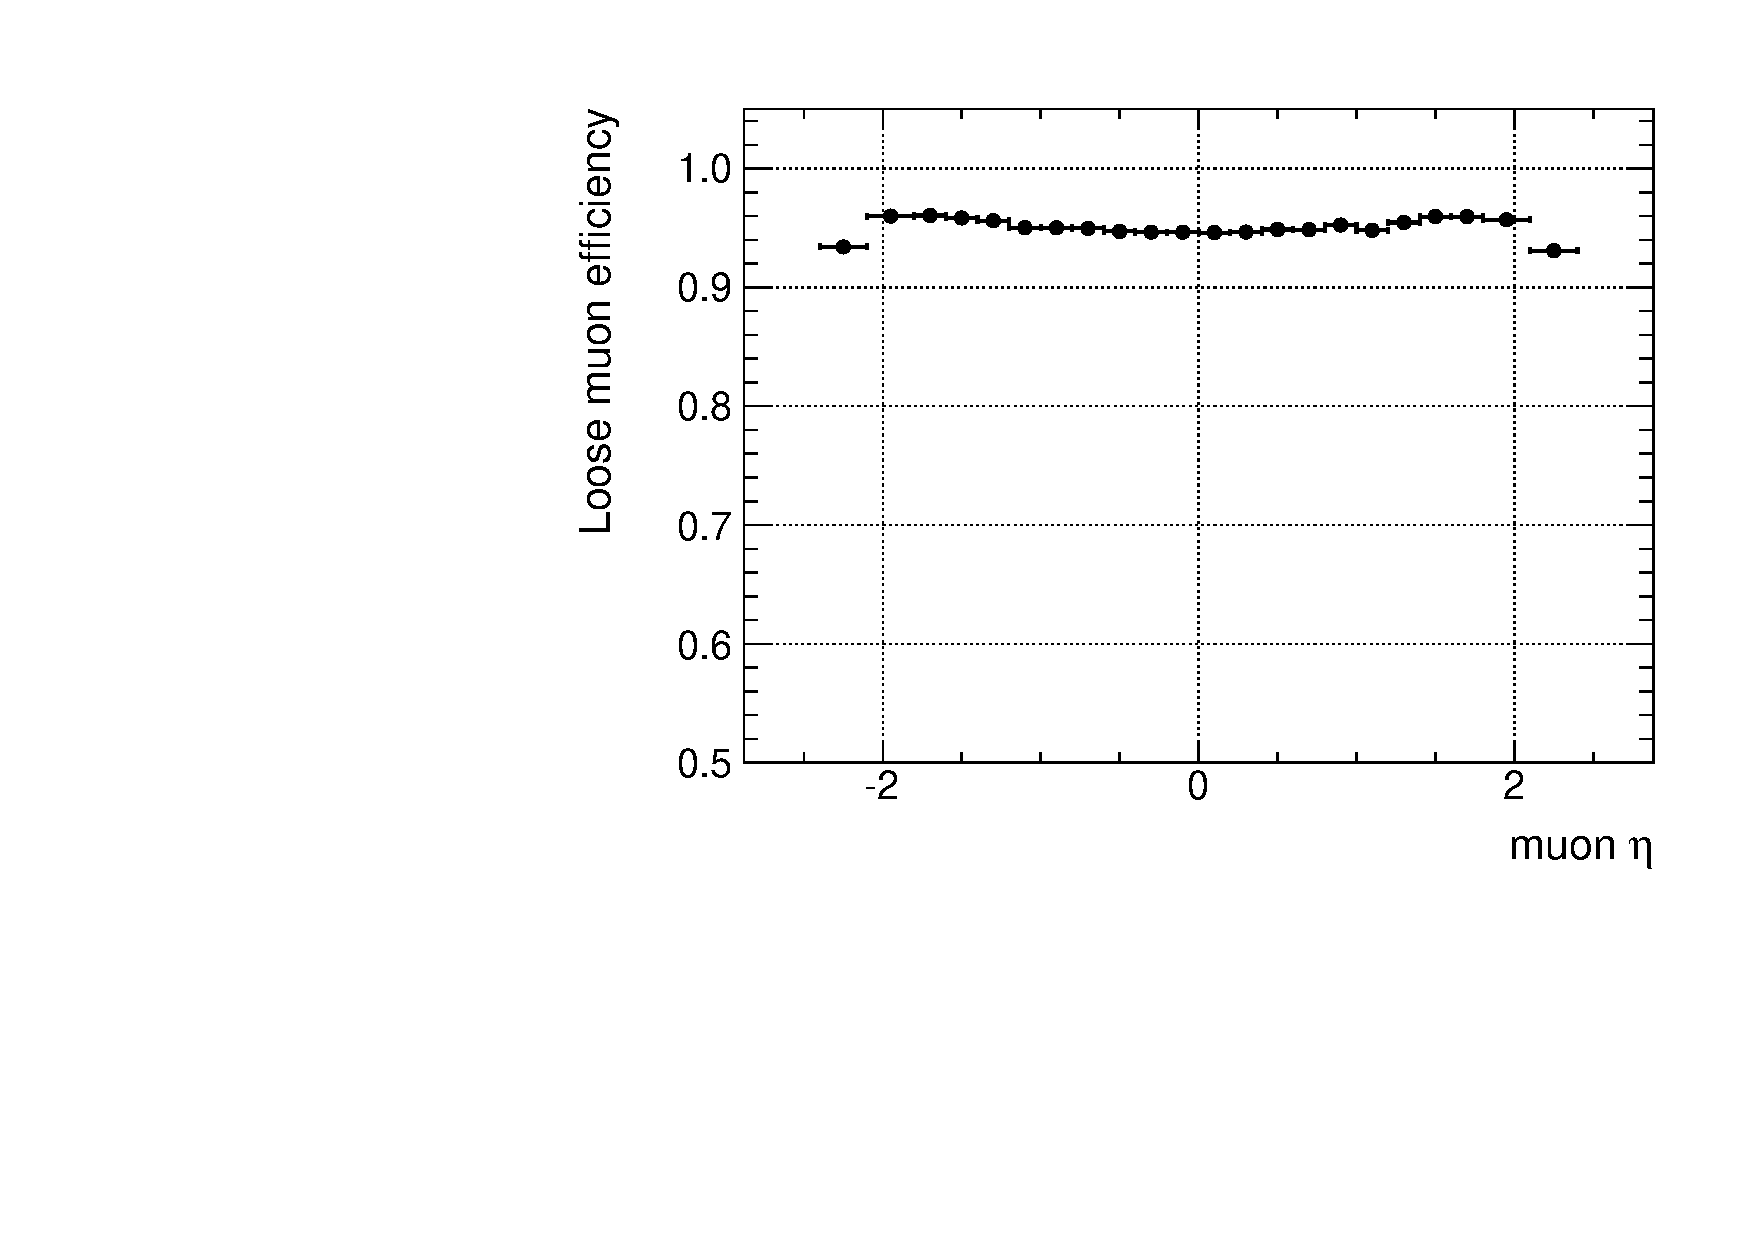
\includegraphics[width=0.48\textwidth]{figures/muloose_effeta.pdf}}
  \subfigure[]{\label{subfig:mulooseeffpt}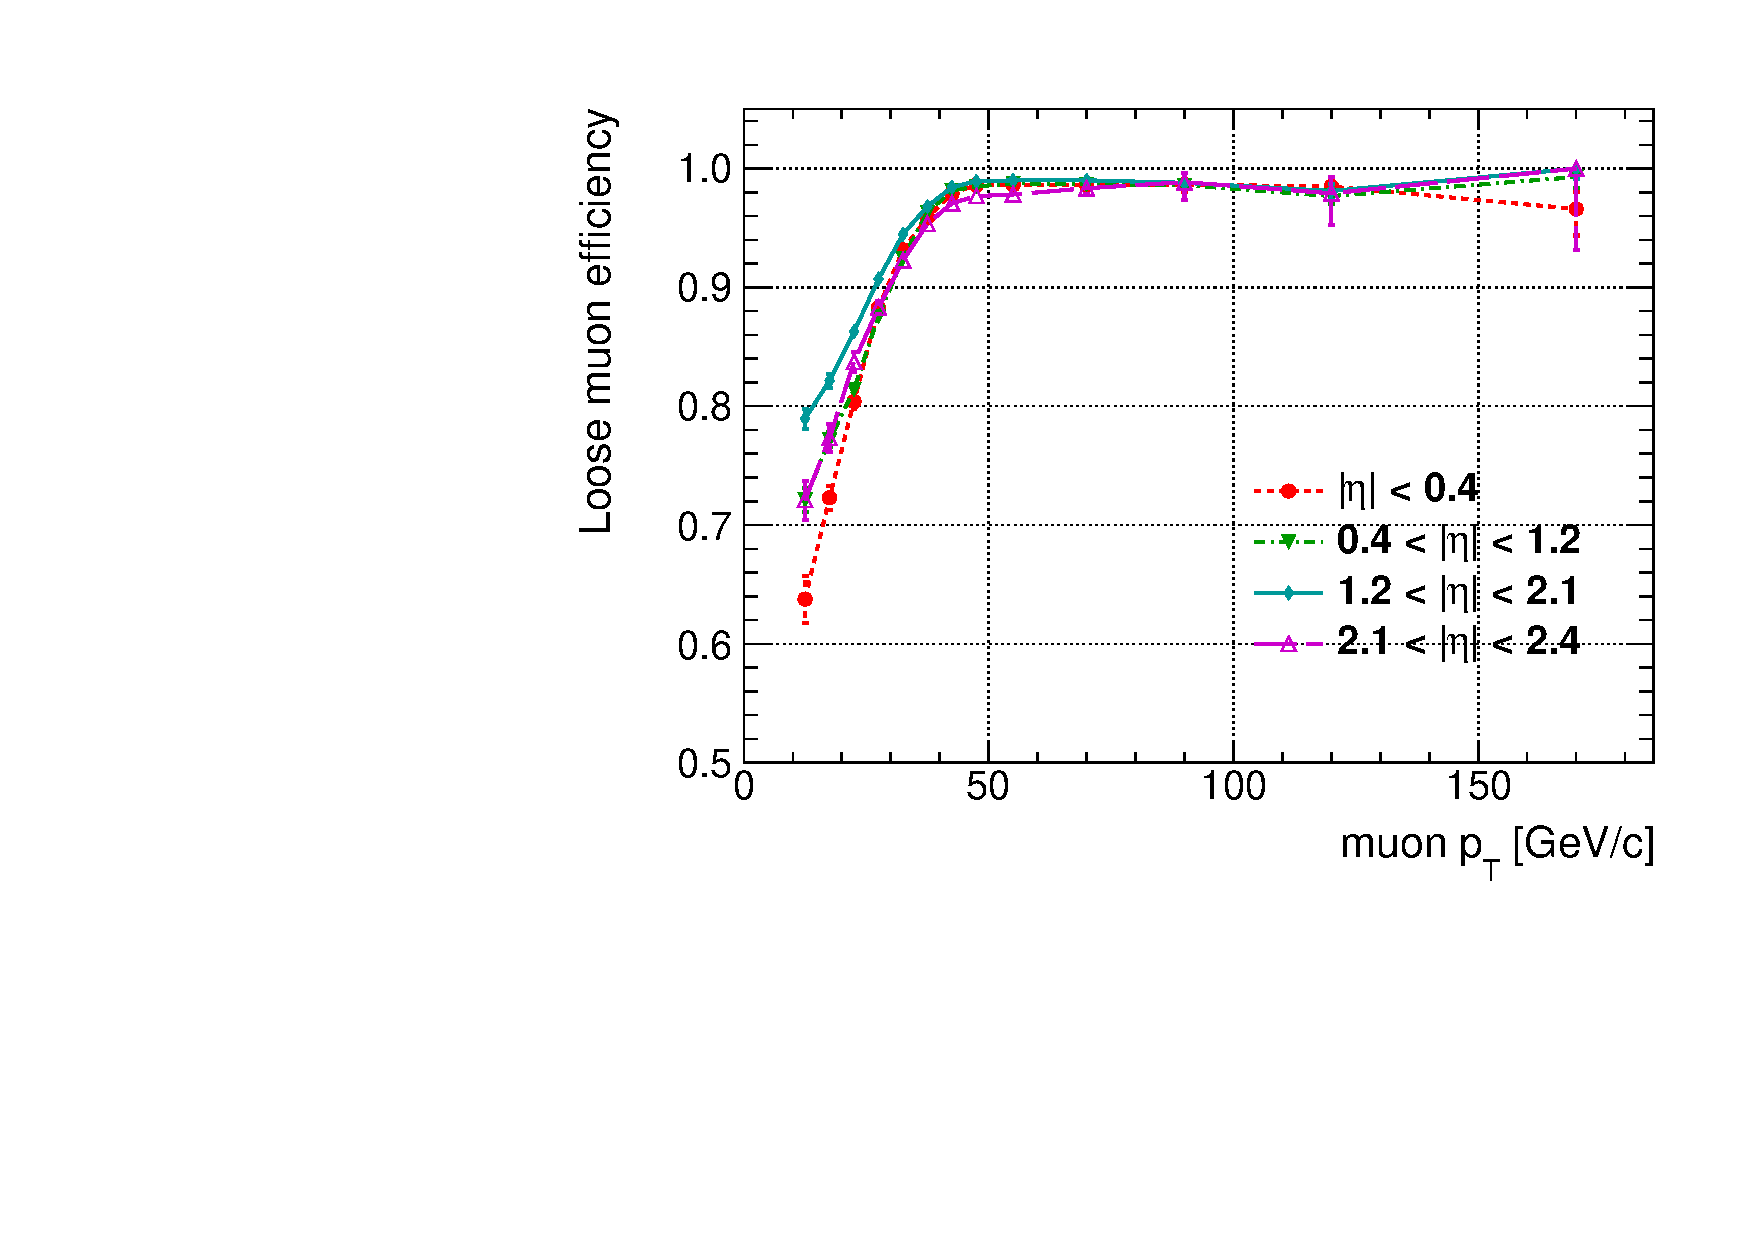
\includegraphics[width=0.48\textwidth]{figures/muloose_effetapt.pdf}}
  \caption{Muon ``Loose'' WP efficiencies with respect to \subref{subfig:mulooseeffeta} $\eta$ and \subref{subfig:mulooseeffpt} $\pt$ in different $|\eta|$-regions.\textcolor{red}{Plots to be updated}}
  \label{fig:mulooseeff}
\end{center}
\end{figure}

\begin{figure}[htbp]
\begin{center}
  \subfigure[]{\label{subfig:mutighteffeta}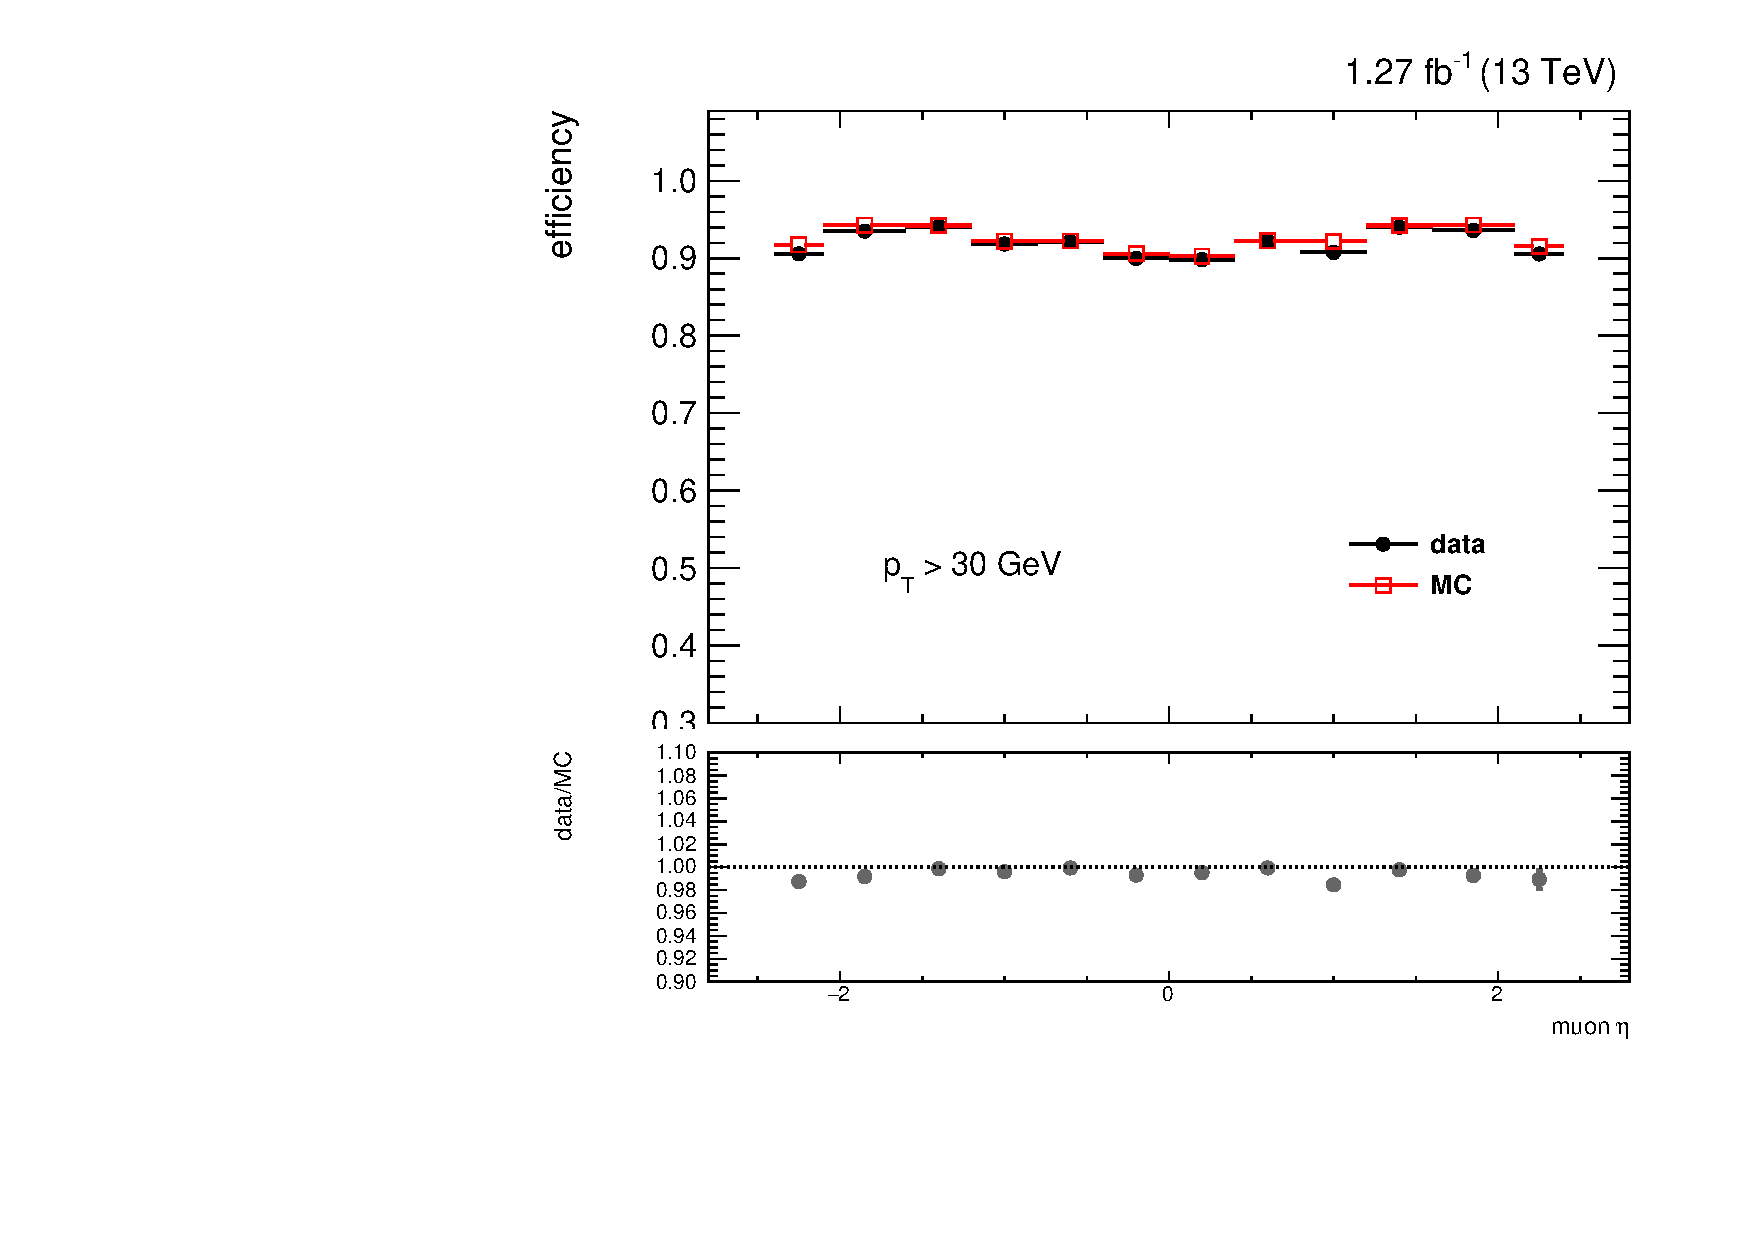
\includegraphics[width=0.48\textwidth]{figures/mutight_effeta_dataMC.pdf}}
  \subfigure[]{\label{subfig:mutighteffpt}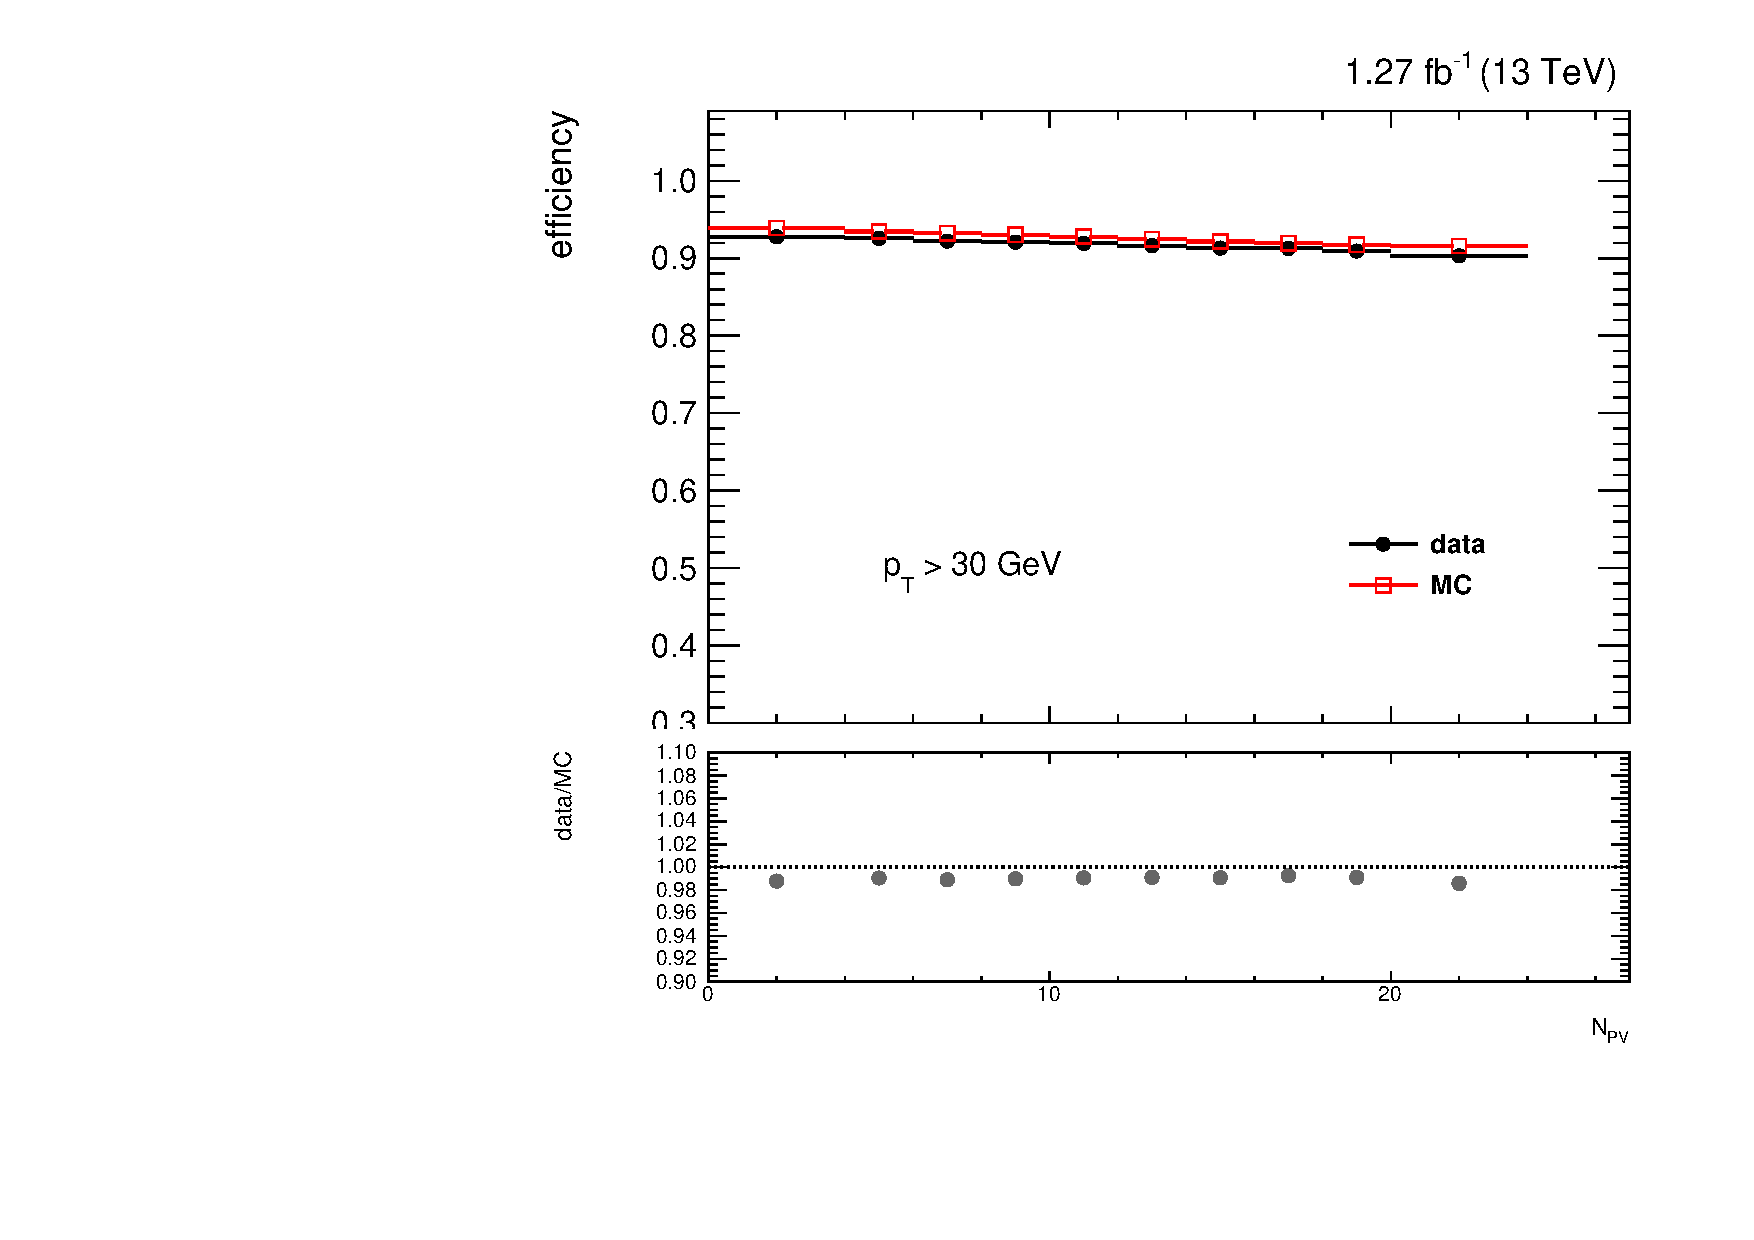
\includegraphics[width=0.48\textwidth]{figures/mutight_effnpv_dataMC.pdf}}
  \caption{Muon ``Tight'' WP efficiencies with respect to \subref{subfig:mutight_effeta_dataMC} $\eta$ and \subref{subfig:mutight_effnpv_dataMC} $N_{PV}$ in data and MC for muons with $\pt>30\:\GeV\:$.}
  \label{fig:mutighteff}
\end{center}
\end{figure}
